\chapter{The Compact Muon Solenoid Experiment at the LHC}
\section{The Large Hadron Collider}

The Large Hadron Collider (LHC) is a double-ring circular synchrotron designed to collide two proton beams with a centre of mass energy $\sqrt{s}$  = 14 $\tev$at a final design luminosity of $10^{34}$cm$^{-2}$s$^{-1}$, with the aim of discovering new physics at the TeV scale. It will also be used to collide heavy lead ions (Pb$^{82+}$) to an energy of 2.76 \tev  per nucleon, in specific runs. In 2011, as part of the early phase of operation the machine was operated at 3.5 TeV per beam, $\sqrt{s} = $7TeV, in order to protect the magnets, and is not expected to run at full energy until 2014. However this energy far surpasses that of its nearest competitor the Tevatron, with 0.98 TeV per beam, and thus holds the world record. This advance allows the investigation for the first time of physics that occurs at the TeV scale, including the search for heavy new particles. The LHC has unparalleled reach in the search for new physics, not only due to the significant increase of energy, but also due to the intensity of the beam delivered. The number of events produced by a given physical process depends proportionally on its cross section $\sigma$, which increases with $\sqrt{s}$, and the luminosity $\lumi$, which has the dependence shown in equation \ref{eq:lumi} below.

\begin{equation}
n = \lumi \sigma, \lumi = \frac{N_{b}^{2} n_{b} f_{rev} \gamma_{r}}{4 \pi \epsilon_{n} \beta^{*}}F
\label{eq:lumi}
\end{equation}


Situated in the tunnel of the previous e+e- machine LEP, spanning the Franco-Swiss border,  the LHC is mostly circular with a circumference of 27km, consisting of 8 arced sectors connected by 8 straight sections in which are the numbered Interaction Points (IP), where the two beams circulating in opposite directions can be allowed to intercept. To accelerate the protons around the rings, the beams must experience opposite dipole fields from one another, and have two separate vacuum systems. As the tunnel has restricted space available, the dipole magnets are twin bore with two coils and, but share the same structure and cryogenics. The superconducting dipole magnets must produce a field in excess of 8T due to the high momentum of the protons, and thus have a high current and must be cooled below 2K by liquid helium to ensure safe operation. The beams are non-continuous, grouped in "bunches" at intervals. At the IPs the two beams are directed to coincide, and quadropole magnets are used to collimate the beam in order to maximise the cross sections. 

At four of these IP's are located the four main detectors that analyse the data from collisions: ATLAS (A Toroidal LHC Apparatus) at IP1 and CMS(Compact Muon Solenoid) at IP 5 are multi-purpose detectors analysing the p-p collisions for signs of new physics. At IP 8 the LHCb (LHC beauty) detector looks for CP violation and other rare decays in a forward detector, and ALICE (A Large Ion Collider Experiment) at IP 2 will investigate the lead-lead ion collisions. The locations of the detectors in the LHC ring is shown in Figure XXX.


The LHC magnets are set up for beams of a certain energy range, and therefore it is not possible to accelerate the particles here from low energies, an acceleration and injection system is required. A beam of 50MeV protons is created in LINAC2, in 6 bunches, and each bunch is then split into 12, resulting in 72 bunches which are fed into the Proton Synchotron Booster. After accelerating to an energy of 1.4GeV, they enter the Proton Synchotron, where they are accelerated to 26GeV, and fed in sets of 2-4 into the Super Proton Synchotron. Now 144-288 bunches, they are accelerated to 460GeV ready of injection into the LHC. Twelve of these sets are injected into the LHC at one, directly into both rings, giving a nominal bunch density of 2808, with a spacing of 25ns. This process takes ~20 minutes, and then the LHC takes a further ~20minutes to ramp up to desired energy. The magnets preventing the beams coinciding in the detectors are turned off and stable collisions occur. The luminosity falls regularly as the run progresses, and after ~10 hours, it has fallen below an acceptable level, and the beam is dumped before repeating the process again. Using these short runs of high luminosity it is possible for the LHC to take vast amounts of data. The 2011 Run delivered 5.727 fb$_{-1}$ data, the first 1.1fb$_{-1}$ of which was delivered by the end of June, and is considered for this thesis.

\section{The Compact Muon Solenoid}

The Compact Muon Solenoid (CMS) is one of the two multi-purpose detectors at the LHC, designed to capitalise on the full range of physics opportunities available at the LHC. These goals are pursued through the design and construction of the detector and development of software for the reconstruction of physics objects. The detector is constructed of several detector sub�-systems contained inside and wrapped in layers around a central 13m long 4T super conducting solenoid as shown in Figure \ref{fig:CMS_Struct}. 

The detector is 21m long, 15m wide and weighs 14000 tonnes, and consists of five wheel-like barrel sections and two end-caps to close. In order for CMS to search for new physics among the high order of Standard Model backgrounds, it is of key importance to develop a detector which has impressive energy and momentum resolution, and particle identification. Different particles interact differently with matter and therefore a number of sub-detectors are needed in order to gather all the relative information. The path travelled by a particle from the interaction point involves the following regions. 

\begin{figure}
\centering
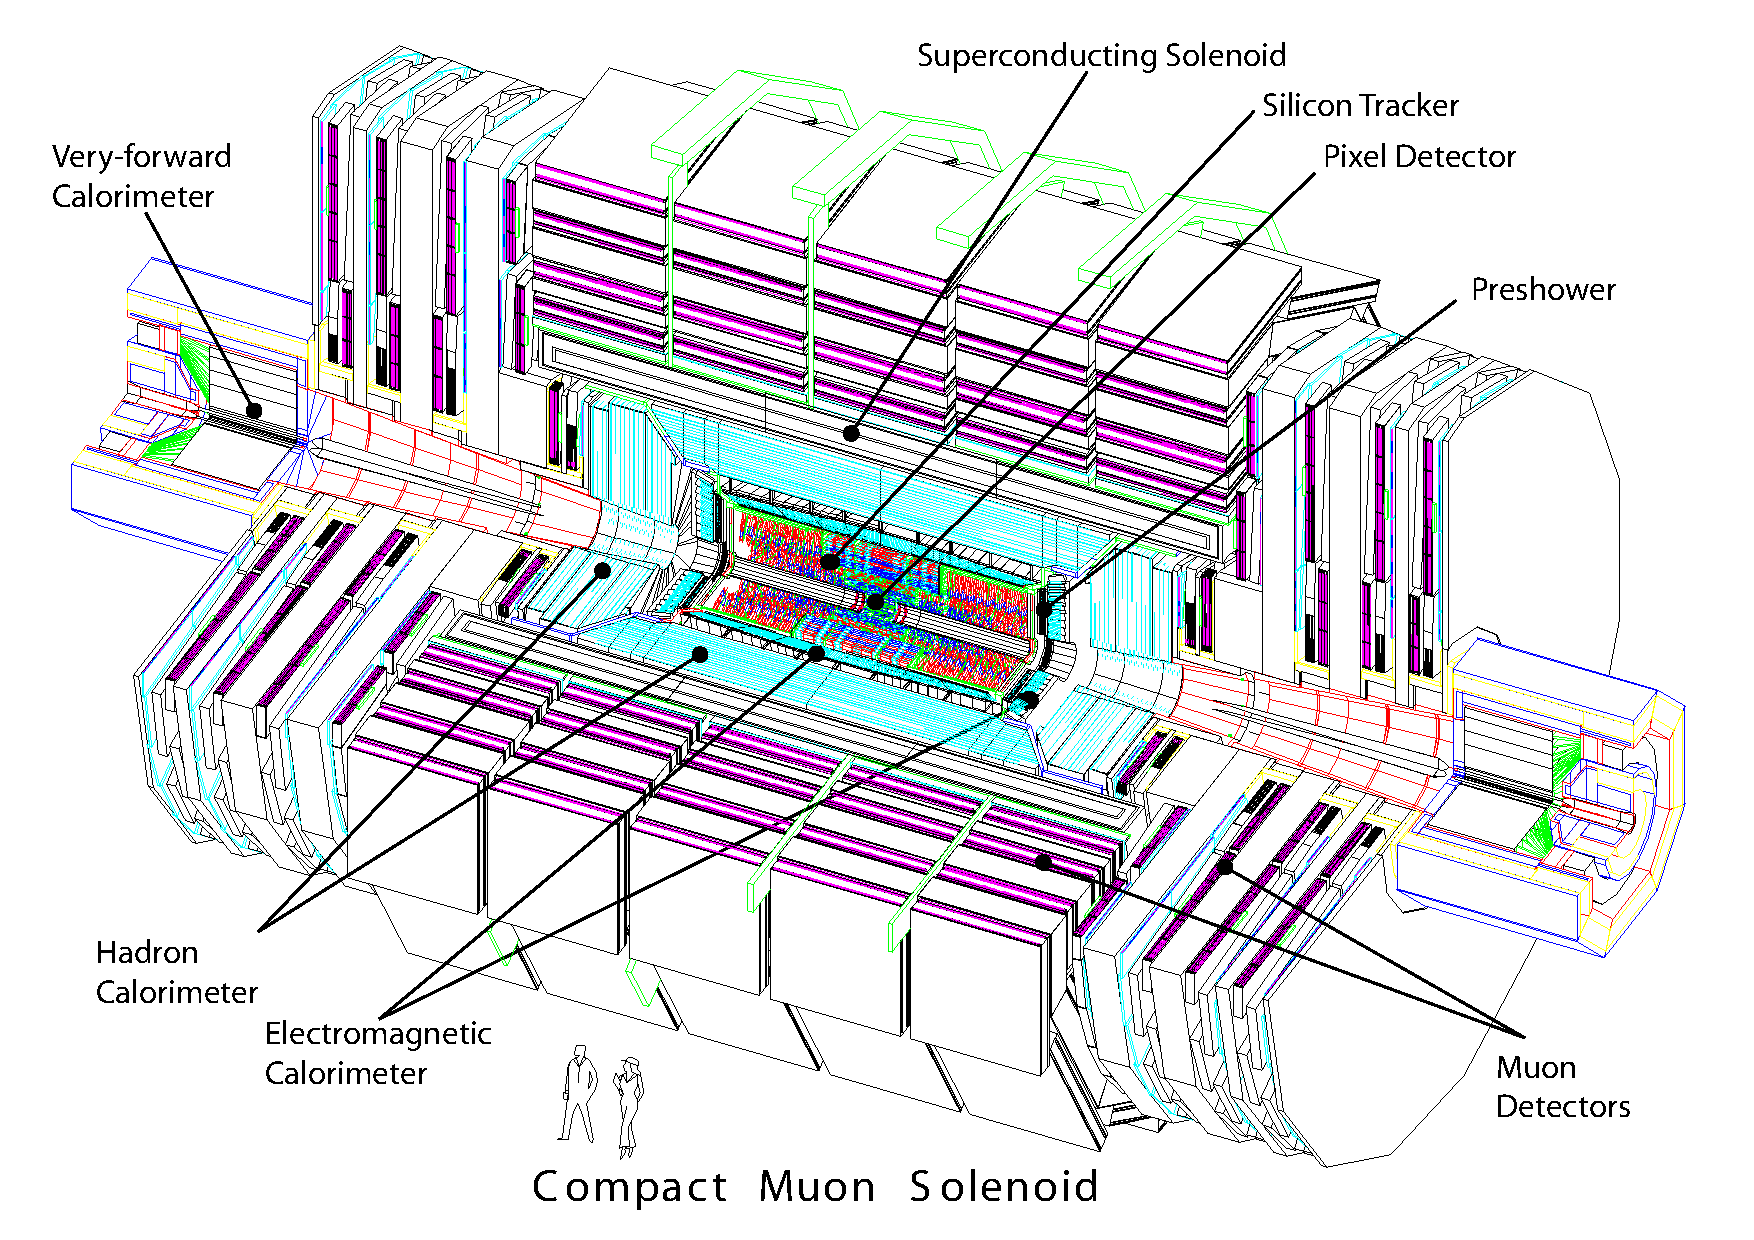
\includegraphics[width=0.8\textwidth]{Figures/Detector/CMS_Structure}
\caption{A cutaway diagram of the CMS detector structure identifying the main individual sub-systems.}
\label{fig:CMS_Struct}
\end{figure}

The high magnetic field was chosen in order to achieve the bending power necessary for good charged particle momentum resolution. The inner bore of the solenoid is large enough that the inner tracker and the calorimeters are located inside, which minimises the material the partials pass through before entering the calorimeters. This allows a good energy measurement. Four muon "stations" of aluminium drift tubes are integrates within the   iron magnetic field return yoke. The full design description can be found in the CMS Technical Design Proposal \cite{CMSTDP}. As different particles pass through the detector they interact in the sub-systems depending on their type. A transverse slice through the detector illustrating the path through the machine of each type of particle is shown in Figure \ref{fig:CMS_Slice} 





\begin{figure}
\centering
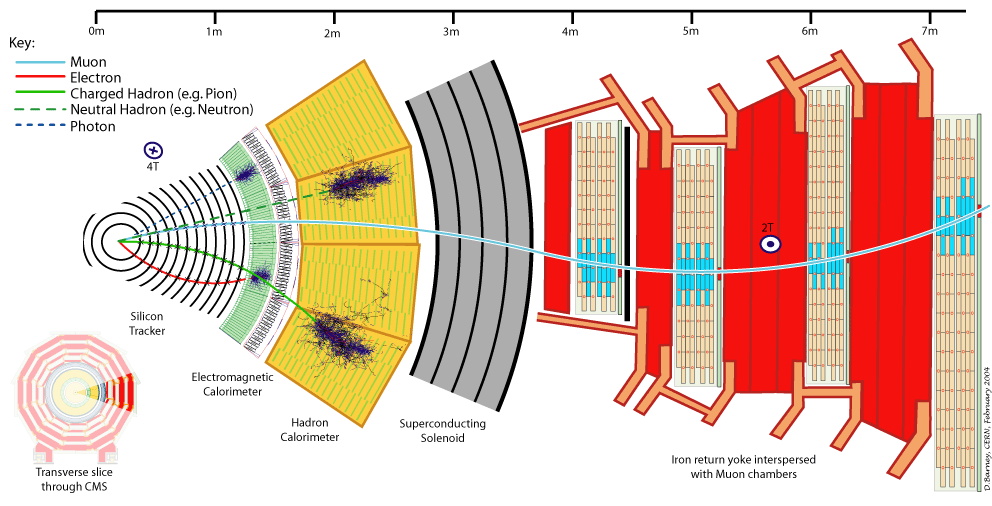
\includegraphics[width=0.8\textwidth]{Figures/Detector/CMS_Slice}
\caption{Transverse slice through the CMS Detector showing each type of particle and how it interacts with the sub-detectors.}
\label{fig:CMS_Slice}
\end{figure}
\subsection{Coordinate System}

The coordinate system chosen by CMS uses the nominal interaction point within the detector as the origin. The x-axis points radially inwards to the centre of the beam pipe, and the y-axis points vertically upward. The z-axis then points in the direction of the beam. The azimuthal angle $\phi$ is defined as the angle from the x-axis in the x-y plane, and the polar angle $\theta$ from the z-axis. However, it is common convention to express $\theta$ in terms of the Lorentz Invariant quantity, pseudorapidity~\begin{math}
\eta = -\ln \tan (\theta / 2) 
\end{math}, as particle production is approximately uniform in $\eta$. The transverse components of the energy and momentum, denoted $E_{T}$ and $p_{T}$ are then calculated form the $x$ and $y$ components. 



\subsection{Superconducting Magnet}

The geometry of the magnetic field is integral to the design and cylindrical structure of the CMS detector, as it uses a global solenoidal magnet. A strong magnetic field is essential to the design of a detector, bending charged particles in order to measure their charge and momentum. In order to ensure that the curvature is significant even with particles of high momentum, the CMS solenoid is designed to be capable of delivering a homogenous field of 4T. Consisting of four layers of NbTi coils, in a vacuum with a cryogenic system maintaining a temperature of 4.5K, the solenoid has a diameter of 5.9m and length 12.5m, and when operating at full current stores 2.6GJ of potential energy.

As the solenoid is so large, not only the inner tracking system but also both calorimeter sub-detectors can be accommodated in the interior, giving significant advantage to electromagnetic and jet energy resolution, as particles will not have traversed the high-density magnet coil before these measurements are taken. The flux is returned with a large iron yoke of $10_(7)kg$, surrounding the inner magnet and built with a barrel of 5 wheels, and two end-caps each containing three disks. The muon system is built within the iron return yoke, in order to take advantage of the reverse magnetic field produced in the outer region, and thus follows the same structure. The drawback of a solenoidal field is that it had strong inhomogenity in the end-caps, affecting the performance of the muon subsystem. 


\subsection{Tracker}



The first sub-detector encountered by particles is the multi-layer silicon tracker, which records precise information about the path of charged particles bending under the magnetic field. It is placed as close to the interaction point as possible in order to distinguish the primary interaction from secondary vertices of particles with significant lifetimes. This is particularly important in the case of identifying B mesons, which can travel a measurable distance before decaying.  

The tracker is divided into regions defined by the radius r from the interaction point, as the expected particle flux decreases rapidly as the radius increases. This is due to the high magnetic field, which causes low momentum particles to have small radial helical trajectories.

Nearest to the primary vertex at 4cm, where the expected particle flux is at its highest ($\sim10^{8} cm^{-2} s^{-1}$) are 66 million silicon pixel detectors of size 100 $\times$150 $\mu m^{2}$, arrayed in three barrel layers and two end-cap disks. This region is laid out to optimise the resolution in determining the vertex position, delivering a granularity of ~10$\mu m$ in the r-$\theta$ plane and ~20$\mu m$ in the r-z plane. Pixel detectors have the advantage of being able to measure all three coordinates of the particle simultaneously. HOwever this requires a huge number of readout channels and drives the costs of construction up. For this reason these are chosen for the innermost region where the flux is highest, while the test of the detector are composed of silicon micro-strip devices. 

Outside of the pixel detector lies the silicon strip tracker, divided into two parts, the Inner and Outer components. The Inner region, immediately outside the Pixel tracker, is composed of four barrel layers and closed with three disks on each end. Use of the silicon strip detectors cuts down the number of channels needed, and this is made our of X in total. Whilst these do now allow a simultaneous 3-coordinate measurement, the layers are constructed at known angles to one another and therefore combined together all three coordinates can be measured. The Outer region is similar and uses the same principles, with 6 barrel layers further apart than in the Inner sector, and closed with 9 end-caps on the end of the barrel. 



\subsection{ECAL}

Immediately outside of the tracker, and still within the magnet core, sits the Electromagnetic Calorimeter (ECAL), used to measure the energy of electrons, photons and pions via the energy they lose through radiation. Electrons lose their energy in the material through bremsstrahlung, and photons by decaying to an electron-positron pair. Using a hermetic homogenous calorimeter of scintillating crystals, this energy can be converted to scintillation light which is picked up by a light sensitive detector. 

The use of high density crystals allows a fast calorimeter which has fine granularity and is radiation resistant, requirements which are essential in the LHC environment. After rigorous research and development, lead tungstate ($PbWO_{4}$) crystals were chosen as the optimal solution to the requirements of LHC operation, due to a number of desirable characteristics. The extremely short radiation length $X_{0}$ = 0.89cm allows the construction of a compact ECAL which therefore can reside within the solenoid, hence reducing the layers of material the particles have already passed through. In addition, the material has a low Moliere radius (2.2cm) meaning the transverse size of the electromagnetic shower is small, leading to good shower position resolution and separation. It is also essential that a fast scintillator is used, in order to distinguish between bunch crossings. In crystals of PbWO$_{4}$ 80\% of the scintillation light is emitted within 25ns, the bunch spacing of the LHC. Finally the crystals are hard to radiation, as their method of scintillation is resistant to radiation damage. 

The ECAL is structurally divided into three distinct regions, the End-caps (EE), the Barrel (EB) and the Preshower (PS), which together cover a pseudorapidity range $|\eta| \leq$3. The ECAL Barrel is a cylindrical arrangement of 61200 PbWO$_{4}$ crystals covering the pseudo rapidity range $|\eta| \leq$ 1.479 with a granularity of $\Delta \eta \times \Delta \phi = 0.0174 \times 0.0174$. The radius to the front-face of the crystals is 1.29 m. 


The ECAL is closed by two identical end-cap regions, which cover the range 1.479 $\leq |\eta| \leq$ 3 at the margins of the barrel, and consist of 7324 crystals each. Both are divided into two halved, or \textit{Dees} Precision energy measurements are possible up to $|\eta|$ = 2.6, but crystals are include up to $|\eta|$ = 3 to assist the forward-direction energy-flow measurement. The end cap crystals are also wedge shaped with a square front face $28.62 \times 28.62 mm^{2}$ and a square back face $30 \times 30 mm^{2}$. The crystals point slightly away from the interaction point in order to make the end-caps hermetic, and are grouped mechanically into 5 $\times$ 5 super-crystals (SC). 

 The size of the crystals is chosen to reflect the properties and requirements, such that the front face surface area is 22mm x 22mm (the size of the Moliere radius) and the longitudinal depth of the crystals is 230mm, which is 25.8 X$_{0}$ in the barrel, hence allowing a fine granularity and a compact ECAL. In the end-caps the presence of the PS allows for shorter crystals, of 220m, corresponding to 24.7 X$_{0}$.

A additional component, the Pre-Shower is present in front of the end-caps covering a range of $1.653\leq |\eta|\leq2.6$ and consists of two layers of absorbing lead converters and silicon detectors. The primary function of the PS is to identify neutral pions that decay into two photons in the end-caps, which can fake a high-energy photon. It also possesses a high granularity, and therefore is used to improve position determination of particles, and helps the identification of electrons against minimum ionising particles. The two layers of the PS have their strips orthogonal to one another such that the first layer has vertical strips to measure the critical position, and the second horizontal strips for the horizontal position. 

The scintillators are read out using photodetectors, which convert the scintillating light of the crystals into an electric signal. The crystals were chosen by a rigorous optimisation of the properties required, which results in a high-performance ECAL, however this material has a relatively low light yield. In order to overcome this, photodetectors designed for use in a magnetic field with intrinsic gain are used. Vacuum Phototriodes  (VPTs) are used in the end-caps. These are unsuitable in the central region due to high magnetic, but due to lower radiation levels Avalanche Photodiodes (APDs) are used. Both the crystals and the photodetectors are sensitive to temperature changes, so a stable temperature must be maintained. Radiation damage to the crystals decreases with temperature, but so do the thermal effects which result in recovery. The operational temperature, 18C is chosen as it is the point of equilibrium between damage and recovery.


The resolution of an ECAL can be described as a function of the energy E in GeV, shown in Equation: \ref{eq:E-Res} \cite{PDG}, for energies below about 500 GeV. Above this shower leakage from the back of the crystals become non-negligible. 
\begin{equation}
\left(\frac{\sigma}{E}\right)^2 = \left(\frac{S}{\sqrt{E}}\right)^2 + \left(\frac{N}{E}\right)^2 + C^2
\label{eq:E-Res}
\end{equation}
The stochastic term S represents fluctuations related to statistics, including photoelectron statistics and intrinsic shower variations. The noise term N takes into account electronic noise summed over readout channels, and the constant term C accounts for the uncertainty in calibration and the detector non-uniformity. Measurements from test beam reconstructed energy distributions show values for the terms to be S\,=\,2.8\,$\pm$\,0.1\,\%, N=0.12\,GeV and C\,=\,0.30\,$\pm$\,0.01\,\%. 


\subsection{HCAL}

Outside the ECAL lies the Hadronic Calorimeter (HCAL),  responsible for the measurement of the hadronic activity of an event. This also leads to a measurement of apparent missing energy from neutrinos or exotic particles, an important quantity in many searches for new physics. In order to measure the energy of hadrons in a compact space, a sampling calorimeter of interleaved layers of absorbers and scintillators is used. The absorbing material forces hadronic showering through nuclear interaction with heavy nuclei, and the active scintillating material then detects samples the showers of charged particles produced. The absorber material is described by the interaction length $\lambda_{I}$, the distance a hadron will travel through the material before it has lost roughly 63\% of its energy through nuclear interactions.

 The HCAL is divided into several sections, dependent on pseudo-rapidity in order to optimise the resolution under different conditions. Within the space between the ECAL and the magnet coil lie the HCAL Barrel (HB) at $|\eta| < 1.305$, and the HCAL End-Caps (HE) at $1.305 < |\eta| < 3.0$, hermetically joined to completely surround the ECAL. In order to increase the hermicity of the HCAL, and therefore improve the accuracy of the missing energy measurement, two forwards calorimeters (HF) overlap with the HE and extend the range in pseudorapidity to $|\eta|<5$. There is also a complimentary layer of scintillators on the outside of the coil, known at the HCAL Outer (HO).  This provides shower containment in the central region, where the number of interaction lengths travelled by a particle is at its lowest, ~5 ~\cite{HCALTDR}.


\begin{figure}
\centering
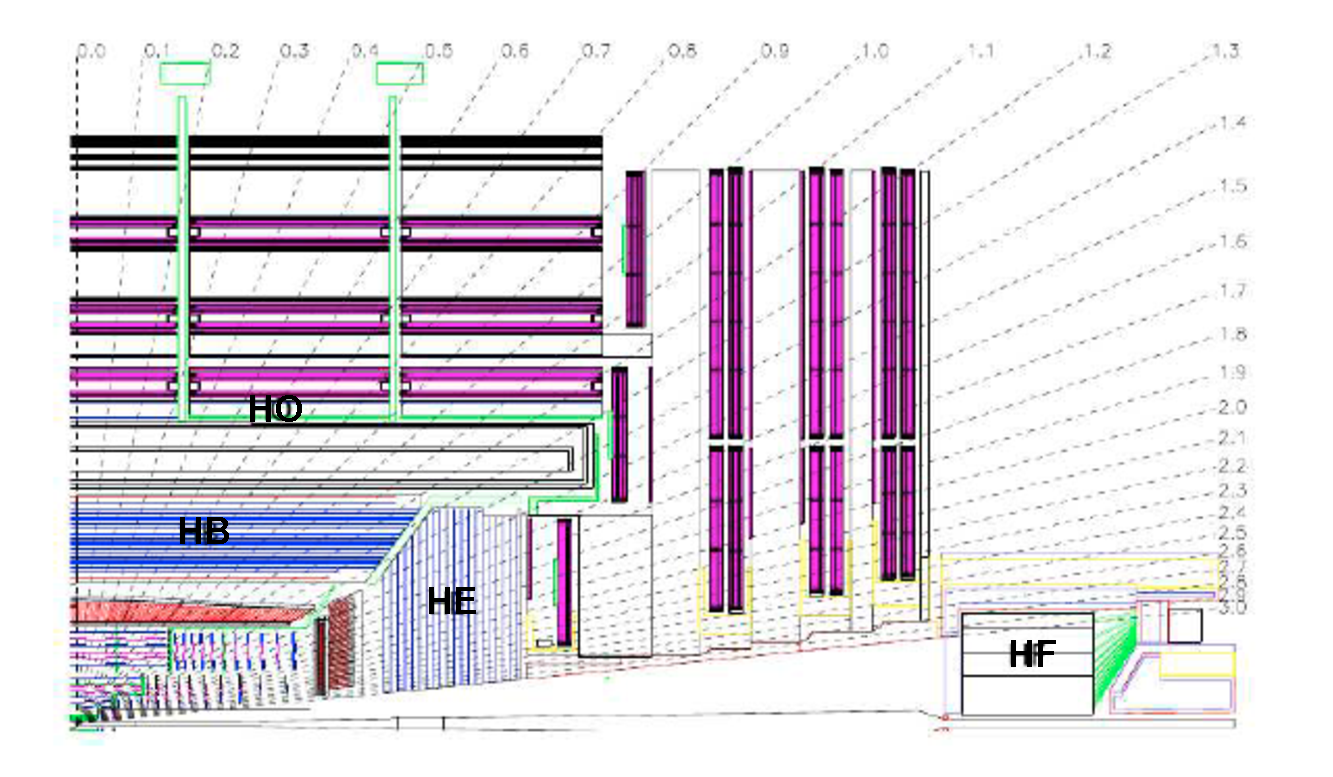
\includegraphics[width=0.8\textwidth]{Figures/Detector/HCAL}
\caption{Diagram showing the locations of the components of the HCAL: HB, HE, HO and HF, in one quarter of the detector.}
\label{fig:HCAL}
\end{figure}


The barrel consists of two halves each with 18 identical azimuthal wedges, extending outwards 0.96m. Each wedge has 17 layers of 3.7mm thick plastic scintillator, interspersed with brass absorber plates, with the exception of the innermost and outermost absorbers, made from stainless steel to add structural stability. Directly behind the ECAL is placed the first active layer, with more than double the scintillator thickness (9mm) to actively sample the articles traversing the support material between the ECAL and HCAL. The final layer also has this thickness to catch showers that form late in the absorber. 

A similar structure makes up the end-caps with 18 wedges in $\phi$ containing 19 active plastic scintillators with brass absorbers between. The number of interaction lengths travelled by particles in the HB and HE is dependent on the $\eta$ of the particle, and while it is 10 at high $\eta$, in the central region this is as low as 5. In order to compensate for this, an outer barrel detector is added, consisting of two layers of scintillating material outside the magnet, and therefore utilising the core as an absorber. This extends the total thickness of the full calorimeter to at least 11.8 interaction lengths. 

The design of the forward calorimeters is driven by the need for radiation hardness, as� the region closest to the beam line has an energy density up to seven times greater than in the central region. Thus absorbers made of stainless steel and active scintillators of quartz fibres are chosen. Twelve $\phi$ wedges are located 11.2m from the point of interaction, with the fibres parallel to the beam.

Measurements of hadron energies in the region $| \eta| < 3.0$ rely not only on the HCAL setup described, as a significant fraction of hadrons with have begun to shower while travelling through the ECAL, which contributes around one interaction length.  The hadronic component of these showers will continue on into the HCAL, but much of the initial electromagnetic activity ca be contained in the ECAL, thus use of measurements in both calorimeters are combined to reconstruct the true energy of a hadron. Using test beams over a range from 2 to 350 GeV/c the resolution for the reconstruction of hadron energy for the HCAL and ECAL combined is given by the following equation~\cite{HCALTestBeam}.
\begin{equation} 
\left(\frac{\sigma}{E}\right)^2 = \left(\frac{84.7\%}{\sqrt{E}}\right)^2 + \left(7.4\% \right)^2 
\label{eq:H-Res}
\end{equation}





\subsection{Muon System}

Interleaved in the iron return yoke of the detector are the components of the Muon System (MS), an important design feature giving CMS its middle initial. Many new physics signatures at high energy have final states with high momentum muons, and therefore accurately measuring these is crucial for many analyses, including Higgs and SUSY channels. As muons have high mass they interact little in the calorimeters, and thus retain a high percentage of their energy by the time they reach the iron return yoke. Putting the MS here far away from the interaction point allows finer precision, utilising the high magnetic field to bend even high momentum muons, and measuring the bending angle.

Muon momentum resolution using the MS is dominated at low energies (0 $< p^{\mu}_{T} < $ 200 GeV/c) by the multiple scattering that occurs in the material prior to the first muon station, and therefore a better resolution could be obtain during the tracking system. However, it is possible to use the muon trajectory after the yoke to extrapolate back to the interaction point. Using the tracker and muon system together improves identification and measurements, especially as any particle detracted in the MS is expected to be a muon, as other particles are stopped earlier in the detector~\cite{MuonTDR}. 

Built within the iron yoke the MS shares the same structural layout, constructed in five barrel wheels, and two end-caps, together covering the region $|\eta| < 2.4$. As a large area must be covered, a silicon based setup such as the inner tracker would be too expensive, hence gaseous detectors are chosen. In the barrel region ($|\eta| < 1.2$)Drift Tubes (DT) are used, and in the end-caps ($0.9 < |\eta| < 2.4$) Cathode Strip Chambers (CSC) are preferred. As gas detectors have a long response time, they are not suitable for use with the trigger, and so a third element is added in both regions, the Resistive Plate Chambers (RPC). The arrangement of the muon system is shown in Figure \ref{fig:MuonSystem}, with the locations of each type of detector shown.

\begin{figure}
\centering
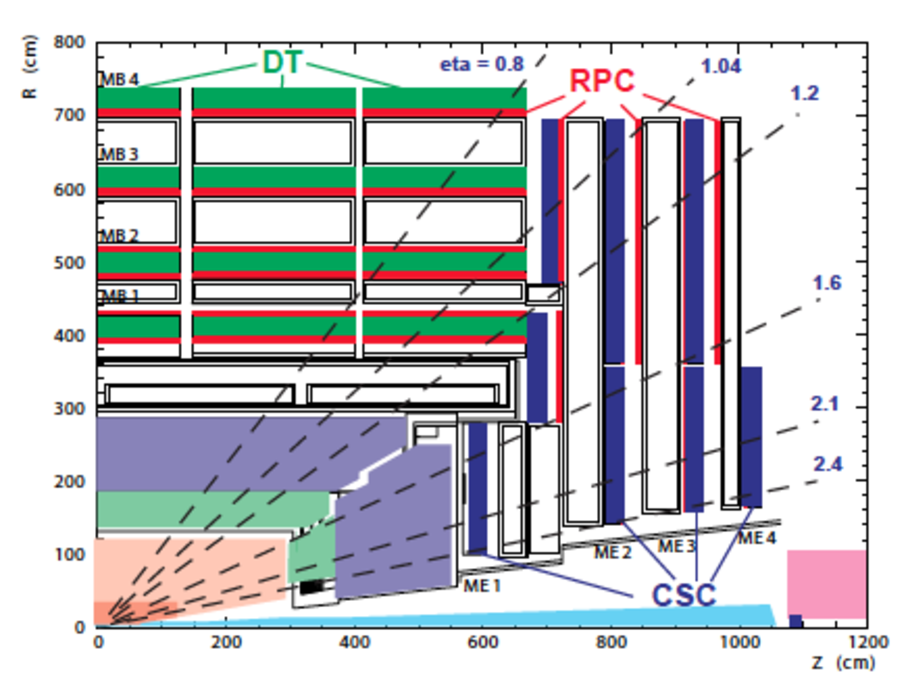
\includegraphics[width=0.8\textwidth]{Figures/Detector/MS}
\caption{The Muon system shown in the $r-\theta$}
\label{fig:MuonSystem}
\end{figure}

In the barrel, the magnetic field is uniform, and therefore allows the use of Drift Tube chambers.  Each of the five wheels are made up of 12 sectors, containing four chambers apiece, making up a full barrel of 240 chambers. The inner three chambers consist of three Super Layers (SL) using the first and third for the $\phi$ coordinate measurement and the second for the z coordinate. In the outer chamber,  there are only two SL's and these contribute only to the $\phi$ measurement. Four layers of drift tubes make up a SL, and each layer is shifted by half a cell from the one beneath, to ensure any particle trajectory meets some active material. Each tube contains an anode wire and cathode strips, and is filled with a gas mixture of 85\% Ar and 15\% $CO_{2}$ gas. The Ar atoms are ionised by a charged particle, and the resulting electrons and ions drift towards the anode and cathodes. Electrons reaching the wire are extremely excited by the high density field, which allows them to ionise further molecules, known as the "avalanche effect". Thus an electrical signal can be measured. The drift distance is XXXX and the drift time is limited to ~380ns by the gas chosen, corresponding to 16 bunch crossings, hence these are not suitable to provide accurate bunch information to the trigger.

Due to the aforementioned solenoidal magnetic field, the end-caps experience an irregular magnetic field, and a higher expected particle flux, and therefore drift tubes are not suitable. In this region 468 Cathode Strip Chambers are used, set out perpendicular  in four stations in each end-cap. Trapezoidal chambers consist of seven radially oriented cathode strips, and in between six planes of azimuthal anode wires. The gas filling the gaps is made up of 40\% Ar, 50\% CO$_{2}$ and 10\% CF$_{4}$, and the chambers work much in the same way as the DT's, with a high voltage applied to achieve the "avalanche effect". As the wires and strips are almost perpendicular its possible to make a simultaneous measurement in r and $\phi$ by identifying the charge fraction in several cathode strips. 

In addition, a complimentary system of RPC's is installed in both the barrel and end-cap regions, providing extra information in the region $|\eta| < 1.6$. In the barrel there are 480 rectangular RPC's, with two layers per station, the inner two stations have one inside and one outside the DT's, and the outer two stations having both inside. The end-caps have overlapping trapezoidal chambers in the outer two concentric rings. These parallel-plate gaseous detectors have two thin gaps between plates, which are attached to high voltage to drive avalanche mode. The avalanche reaches the plates quickly, as the gas gaps have a small width, and so the measurement is made within ~ ns, much smaller than the bunch crossing. The position resolution is adequate at the same time, and so the RPC's are used to contribute to the trigger, and also to map identified muons to a particular bunch crossing.

\subsection{Trigger}

When running at design luminosity, the LHC will collide protons with a bunch crossing of 25ns, each of which will result in ~20 interactions corresponding to a rate of 40MHz of data, or 40 TB/second~\cite{TRIGTDR}. Not only is it impracticable for this volume of data to be stored, but much of this corresponds to unwanted events, where no new particles have been produced, as the cross-sections for interesting physics processes are several magnitudes lower than the inelastic p-p cross section. Hence these events must be whittled into those which it is worthwhile to store and consider, which is done by the trigger system. This is divided into two components, the online hardware-based Level 1 Trigger (L1) to reduce the rate to that which can be routed from the buffer to the computing farm, and then the offline software-based High Level Trigger (HLT). 

The L1 trigger is driven by the amount of time that data at the incoming rate that can be stored in the buffer, before needing to be overwritten. At design luminosity this is 128 bunch crossings, ~3ns. Within this time the rate must be lowered to 10kHz, the acceptable rate for writing to the computing farm used for the HLT. This is accomplished using a tree system of triggers. First, the Regional Calorimeter Trigger (RCT) and Regional Muon Trigger (RMT) undergo local reconstruction of objects (muons, electrons, photons, jets). The Global Calorimeter Trigger (GCT) and the Global MUon Trigger (GMT) receive these objects, and sort them using a number of criteria e.g. Energy, momentum, quality of identification. The top four of each type are sent to the Global Trigger, which uses this information along with global event measurements such as total momentum to decide if the event passes an L1 Trigger requirement. If so it is sent to the HLT, if not it is not stored and passes out of the buffer. 

The HLT essential does the same thing as the L1 trigger, but is not driven by strict time requirements. Running on a large computer farm of multi-core computers, it has access to the entire readout data, and performs sophisticated calculations akin to those performed in physics analyses. Using partial reconstruction algorithms to clearly identify what objects are in an event, it is possible to filter according to a set of desired physics criteria.  The desired rate to store to tape is 100Hz, and the HLT is designed and monitored constantly during data-taking to ensure the correct rate is achieved. In a given run a "menu" of different trigger paths is included, to select different types of event and with different thresholds. Some require the presence of a certain object, such as a Muon. Others combine requirements, and these are called Cross-Triggers. For example a family of triggers exist that require a certain HT and MHT. Within this family there are several different thresholds, which go down as low as can be included in the menu without raising the rate prohibitively much. Thresholds that have a rate which is too high become "pre scaled"



